\section{Теоритические сведения}
Осциллограф~--- регистрирующий прибор, в котором исследуется электрический сигнал
(напряжение) преобразуется в видимый на экране график величины сигнала от времени.

В лабораториях используются электронно-лучевые и цифровые осциллографы.

В электронно-лучевом осциллографе входной сигнал подаётся на отклоняющие конденсаторы,
вызывающие пропорциональные отклонение пучка электронов, попадающих на люминофор
электронно-лучевой трубки (см рисунок) и вызывающих его свечение.

\begin{figure}[ht!]
    \centering
    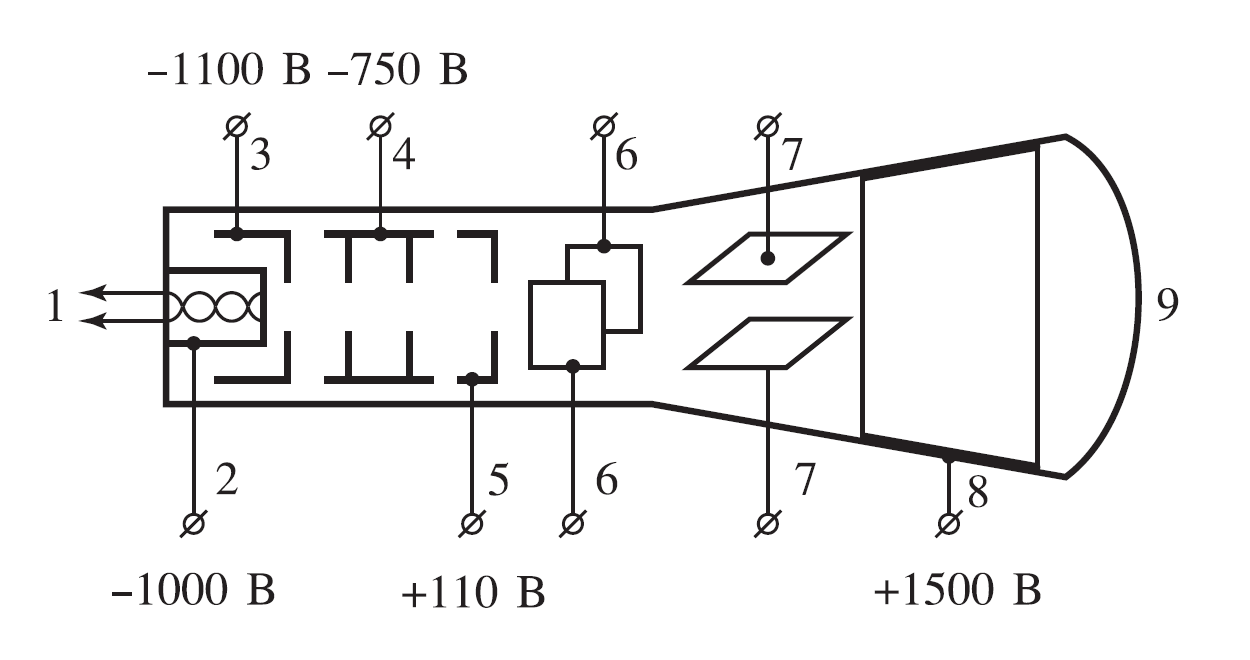
\includegraphics[width=0.8\linewidth]{img/picture1.png}
\end{figure}

Электронно-лучевая трубка представляет собой колбу, откаченную до высокого вакуума,
в которой расположены подогреватель катода 1, катод 2, модулятор 3, фокусирующий
анод 4, ускоряющий анод 5, горизонтально и вертикально отклоняющие конденсаторы 6 и 7,
ускоряющий анод 8, экран 9, покрытый флюоресцирующим веществом.

Подавая на отклоняющие пластины переменное напряжение, можно рисовать электронным
пучком на экране. 

В цифровых приборах аналоговый сигнал преобразуется в цифровой и обрабатывается
компьютером.

Оба типа осциллографов не могут регистрировать колебания с частотами более $1\,\text{ГГц}$.
В электронным осциллографах это связано с конечным временем пролёта электрона от катода до
экрана, а в цифровых~--- с конечной тактовой частотой схем. На самом деле максимальная
частота колебаний ,регистрируемых электронным осциллографом гораздо меньше $1\,\text{ГГц}$,
потому что сигнал надо усиливать и усилители плохо усиливают его на высоких частотах.
Диапазон частот, на котором осциллограф правильно отображает исследуемый сигнал, называется
полосой пропускания.

Смещение луча относительно центра по вертикали и горизонтали пропорционально напряжению
на вертикальном и горизонтальном конденсаторе. Чтобы отклонение луча было заметным и он не
выходил за пределы экрана, сигнал, идущий на пластины конденсаторов, усиливается или
ослабляется.

Для получения изображение на экране нужно на вертикальные пластины подать сигнал, а на
горизонтальные пилообразное напряжение развёртки (см. рисунок).

\begin{figure}[ht!]
    \centering
    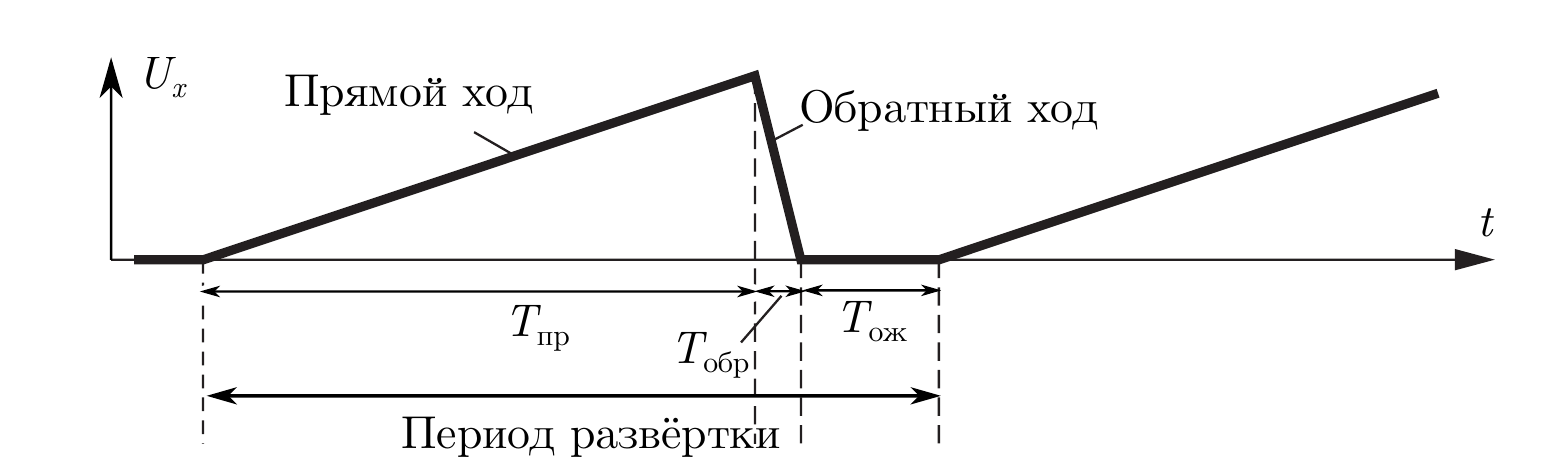
\includegraphics[width=0.8\linewidth]{img/picture2.png}
\end{figure}

Это напряжение генерирует внутренний генератор. В течении времени прямого хода
напряжение изменяется до максимального так, что луч идёт равномерно. Потом в течении
времени обратного хода луч быстро возвращается назад. Потом в течении времени ожидания
луч находится в покое и отрисовка сигнала синхронизируется.

При исследовании периодических сигналов необходимо получить неподвижное изображение.
Для этого период развёртки должен быть кратен периоду изучаемого сигнала. В осциллографе
генератор развёртки сам выбирает частоту изучаемого сигнала и работает на ней.

Наиболее часто синхронизация генератора с сигналом происходит по уровню.
Сначала выставляется пороговый уровень сигнала (уровень синхронизации).
После попадания в режим ожидания прямая развёртка не запускается до тех пор, пока не
произойдёт пересечение уровня. Регулировка уровня позволяет выбрать фазу сигнала в начале
развёртки.

Обычно предусмотрены два режима работы генератора развёртки: автоматический и ждущий.
В ждущем генератор не запускается пока не произойдёт пересечение уровня. В автоматическом
если некоторое время не происходит пересечение уровня, то генератор запускается без синхронизации.

Синхронизировать развёртку можно не только исследуемым сигналом.

\begin{figure}[ht!]
    \centering
    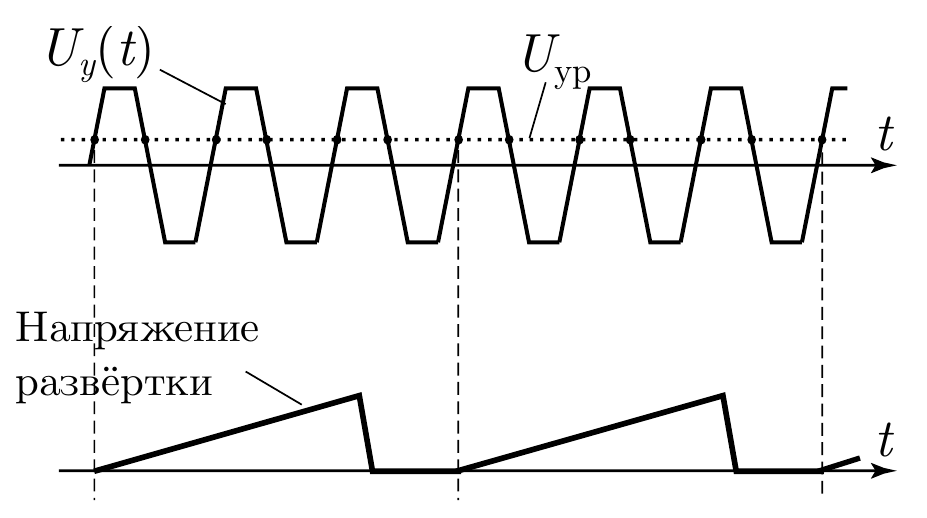
\includegraphics[width=0.8\linewidth]{img/picture3.png}
\end{figure}

Осциллограф также обладает АЧХ и ФЧХ. В широком диапазоне измерений (в полосе пропускания)
АЧХ и ФЧХ~--- константы. Границы полосы пропускания определяются так, что в них АЧХ
меньше своего максимального значения в $\sqrt{2}$ раз. Зависимость АЧХ и ФЧХ от частоты
может приводить к существенным искажениям изображения.

Входные каналы осциллографа могут работать в открытом (AC) и закрытом (DC) режимах.
В закрытом режиме последовательно яко входу подключается конденсатор, который
убирает постоянную составляющую напряжения. В открытом режиме сигнал передаётся
без изменений. В закрытом режиме сильгно искажаются низкочастотные колебания.
Осциллограф обладает большим внутренним сопротивлением.

При совместной подаче сигналов на вертикальные ($U_y$) и горизонтальные ($U_x$)
конденсаторы сигналов
\begin{gather*}
    U_y(t) = U_{0y}\sin \left(2\pi\nu_yt + \varphi_y\right) \\
    U_x(t) = U_{0x}\sin \left(2\pi\nu_xt + \varphi_x\right)
\end{gather*}
можно получить кривые, называемые фигурами Лиссажу (см. рисунок).

\begin{figure}[ht!]
    \centering
    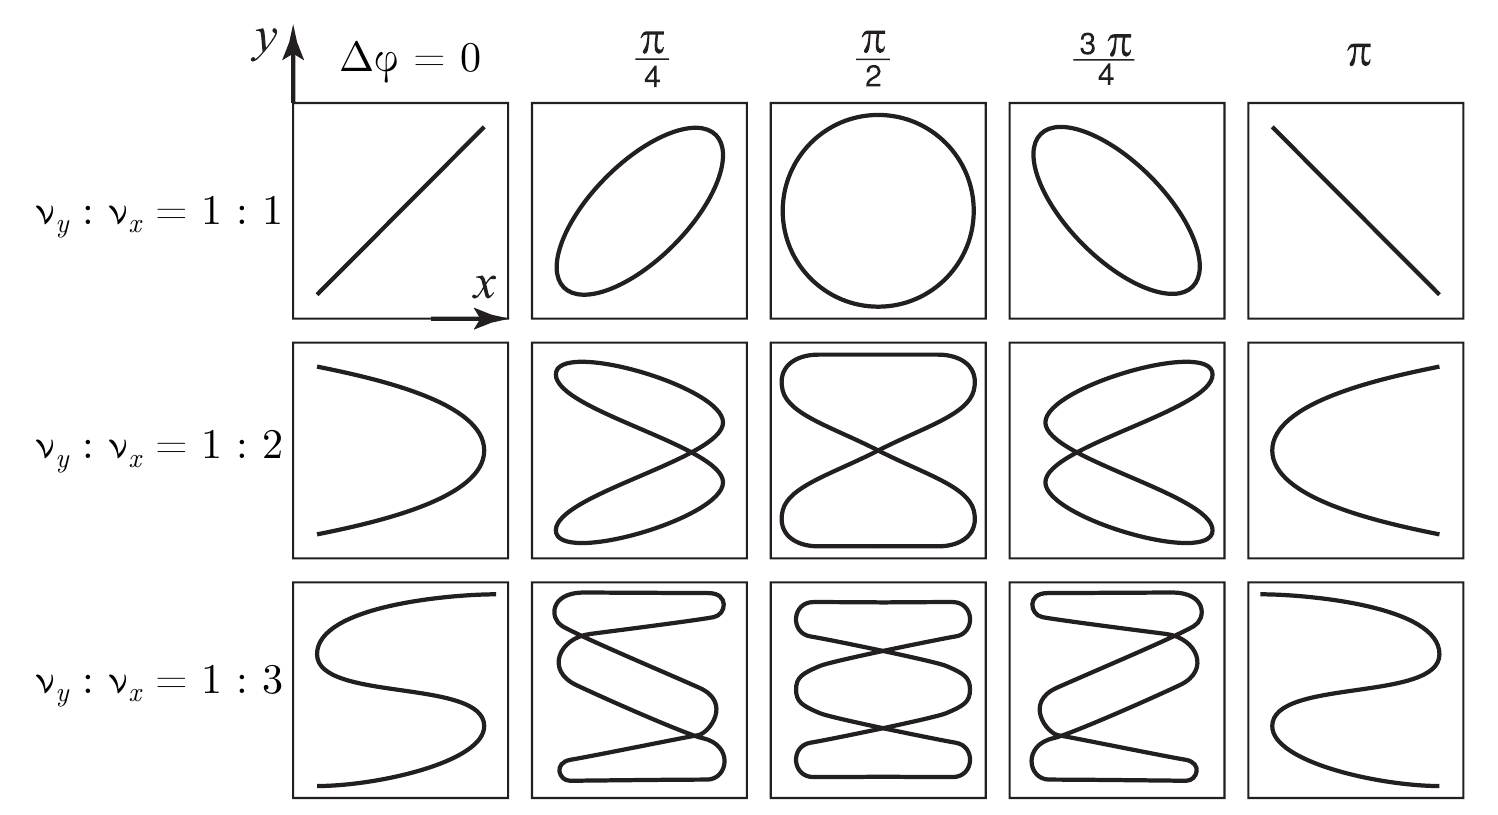
\includegraphics[width=0.8\linewidth]{img/picture4.png}
\end{figure}
